\documentclass[12pt,a4paper]{article}
%----------------------------------------
% German language
% \usepackage[ngerman]{babel}
%----------------------------------------
% Input in UTF8 accepted
\usepackage[utf8]{inputenc}
%----------------------------------------
% Math-packages
\usepackage{mathtools}
\usepackage{amsmath}
\usepackage{amssymb}
%----------------------------------------
% Design choices (?)
%\usepackage{scrlayer-scrpage}
%\pagestyle{scrheadings}
% \clearscrheadfoot
%----------------------------------------
% Footnotes in tables
\usepackage{tablefootnote}
%----------------------------------------
%----------------------------------------
% no parindent
\usepackage{parskip}
\setlength{\parindent}{0em}
%----------------------------------------
% different gap between paragraphs
\setlength{\parskip}{1.3ex}
%----------------------------------------
% spacing between lines
\usepackage[onehalfspacing]{setspace}
%----------------------------------------
% Hurenkinder und Schusterjungen vermeiden
\clubpenalty = 10000
\widowpenalty = 10000
\displaywidowpenalty = 10000
%----------------------------------------
% Geometry package
\usepackage{geometry}
\geometry{
	paper=a4paper, % Change to letterpaper for US letter
	top=3cm, % Top margin
	bottom=3cm, % Bottom margin
	left=3cm, % Left margin
	right=3cm, % Right margin
	%showframe, % Uncomment to show how the type block is set on the page
}
%----------------------------------------
% References
\usepackage[backend=biber, maxbibnames=99, sortcites=true]{biblatex}
\addbibresource{../references.bib}
%----------------------------------------
\usepackage{graphicx}
\graphicspath{ {../assets/images/} }
%----------------------------------------
\usepackage[nottoc]{tocbibind}
%----------------------------------------
\usepackage[onehalfspacing]{setspace}
%----------------------------------------
% formats text "better"
\usepackage{microtype}
%----------------------------------------
% "better" tables
\usepackage{booktabs}
\usepackage{tabularx}
\usepackage{multirow}
\usepackage{makecell}
% for big tables
\usepackage{adjustbox}
%----------------------------------------
%Colours:
\usepackage[dvipsnames, table]{xcolor}
%----------------------------------------
% Definition Box
\usepackage[framemethod=TikZ]{mdframed}
\mdfdefinestyle{enviStyle}{
	innertopmargin = 10pt,
	linewidth      = 1pt,
	frametitlerule = true,
	roundcorner    = 2pt%
}
\usepackage{sectsty}
\newenvironment{CountingDefinition}[2][]{%
	\vspace*{1.7ex}
	\ifstrempty{#1}%
	{\mdfsetup{%
			frametitle={{\strut ~}}}
	}%
	{\mdfsetup{%
			frametitle={{\strut ~#1}}}%
	}%
	\mdfsetup{
		nobreak                   = true,
		linecolor                 = MidnightBlue,
		frametitlebackgroundcolor = MidnightBlue!50,
		style                     = enviStyle
	}
	\begin{mdframed}[]\relax%
		\label{#2}}{\end{mdframed}}
	%----------------------------------------
% Design
%\sectionfont{\color{RedViolet}}
%\subsectionfont{\color{RedViolet}}
\renewcommand{\labelitemi}{$\textcolor{MidnightBlue}{\bullet}$}
\renewcommand{\labelitemii}{$\textcolor{MidnightBlue}{\circ}$}
\renewcommand{\labelitemiii}{$\textcolor{MidnightBlue}{\diamond}$}
\renewcommand{\labelitemiv}{$\textcolor{MidnightBlue}{\ast}$}
%----------------------------------------
% Position figures, etc.
\usepackage{float}
%----------------------------------------
% Lines and dotted lines and other designs
\usepackage{dashrule}
\usepackage{tikz}
\usepackage{tikzpagenodes}
%----------------------------------------
%----------------------------------------
% Hyperref package
\usepackage{hyperref}
\hypersetup{
	colorlinks=true,
	linkcolor=black,
	filecolor=black,      
	urlcolor=MidnightBlue,
	citecolor=black
}
% To include the README files:
%\usepackage{markdown}



%----------------------------------------------------------------------------
%----------------------------------------------------------------------------

\begin{document}
	
% \pagenumbering{roman}




\section{Solutions in Melt Framework?}




\subsubsection*{MLT}

\begin{itemize}
	\item Read through MLT FX User Guide \cite{mltfx}
	
	
	\item[]
	\item Can MLT FX be used in the terminal/through commands or is it an application with UI only? Look into \url{https://www.mltframework.org/docs/fxcut/}? on FX Cut (but this page is from 2005)
	
	
	\item[]
	\item Apply filter?
	\item Look into \url{https://www.mltframework.org/plugins/PluginsFilters/}?
	\item \texttt{melt [options] [producer [name=value]* ]+
		Options:
		\begin{itemize}
			\item[-] attach filter[:arg] [name=value]*       Attach a filter to the output
			\item[-] attach-cut filter[:arg] [name=value]*   Attach a filter to a cut
			\item[-] attach-track filter[:arg] [name=value]* Attach a filter to a track
		\end{itemize}}
	\item Collected information about melt \url{https://superuser.com/questions/358082/command-line-video-editing-in-linux-cut-join-and-preview}
	\item Promising sounding filters:
	
	\newpage
	
		\item
		
		\texttt{avfilter.colorbalance}
		
		\url{https://www.mltframework.org/plugins/FilterAvfilter-colorbalance/}
		
		\texttt{title: colorbalance \newline
			media types: Video \newline
			description: Adjust the color balance.}
		
		$\rightarrow$ looks promising
		
		
		Execution of \texttt{melt https://s3.eu-central-1.amazonaws.com/accurate-player\--demo-assets/timecode/sintel-2048-timecode-stereo.mp4 \\ -filter avfilter.colorbalance av.rs=1 av.gm=1 av.bh=1}:
		
		
		\begin{minipage}{0.5\textwidth}
			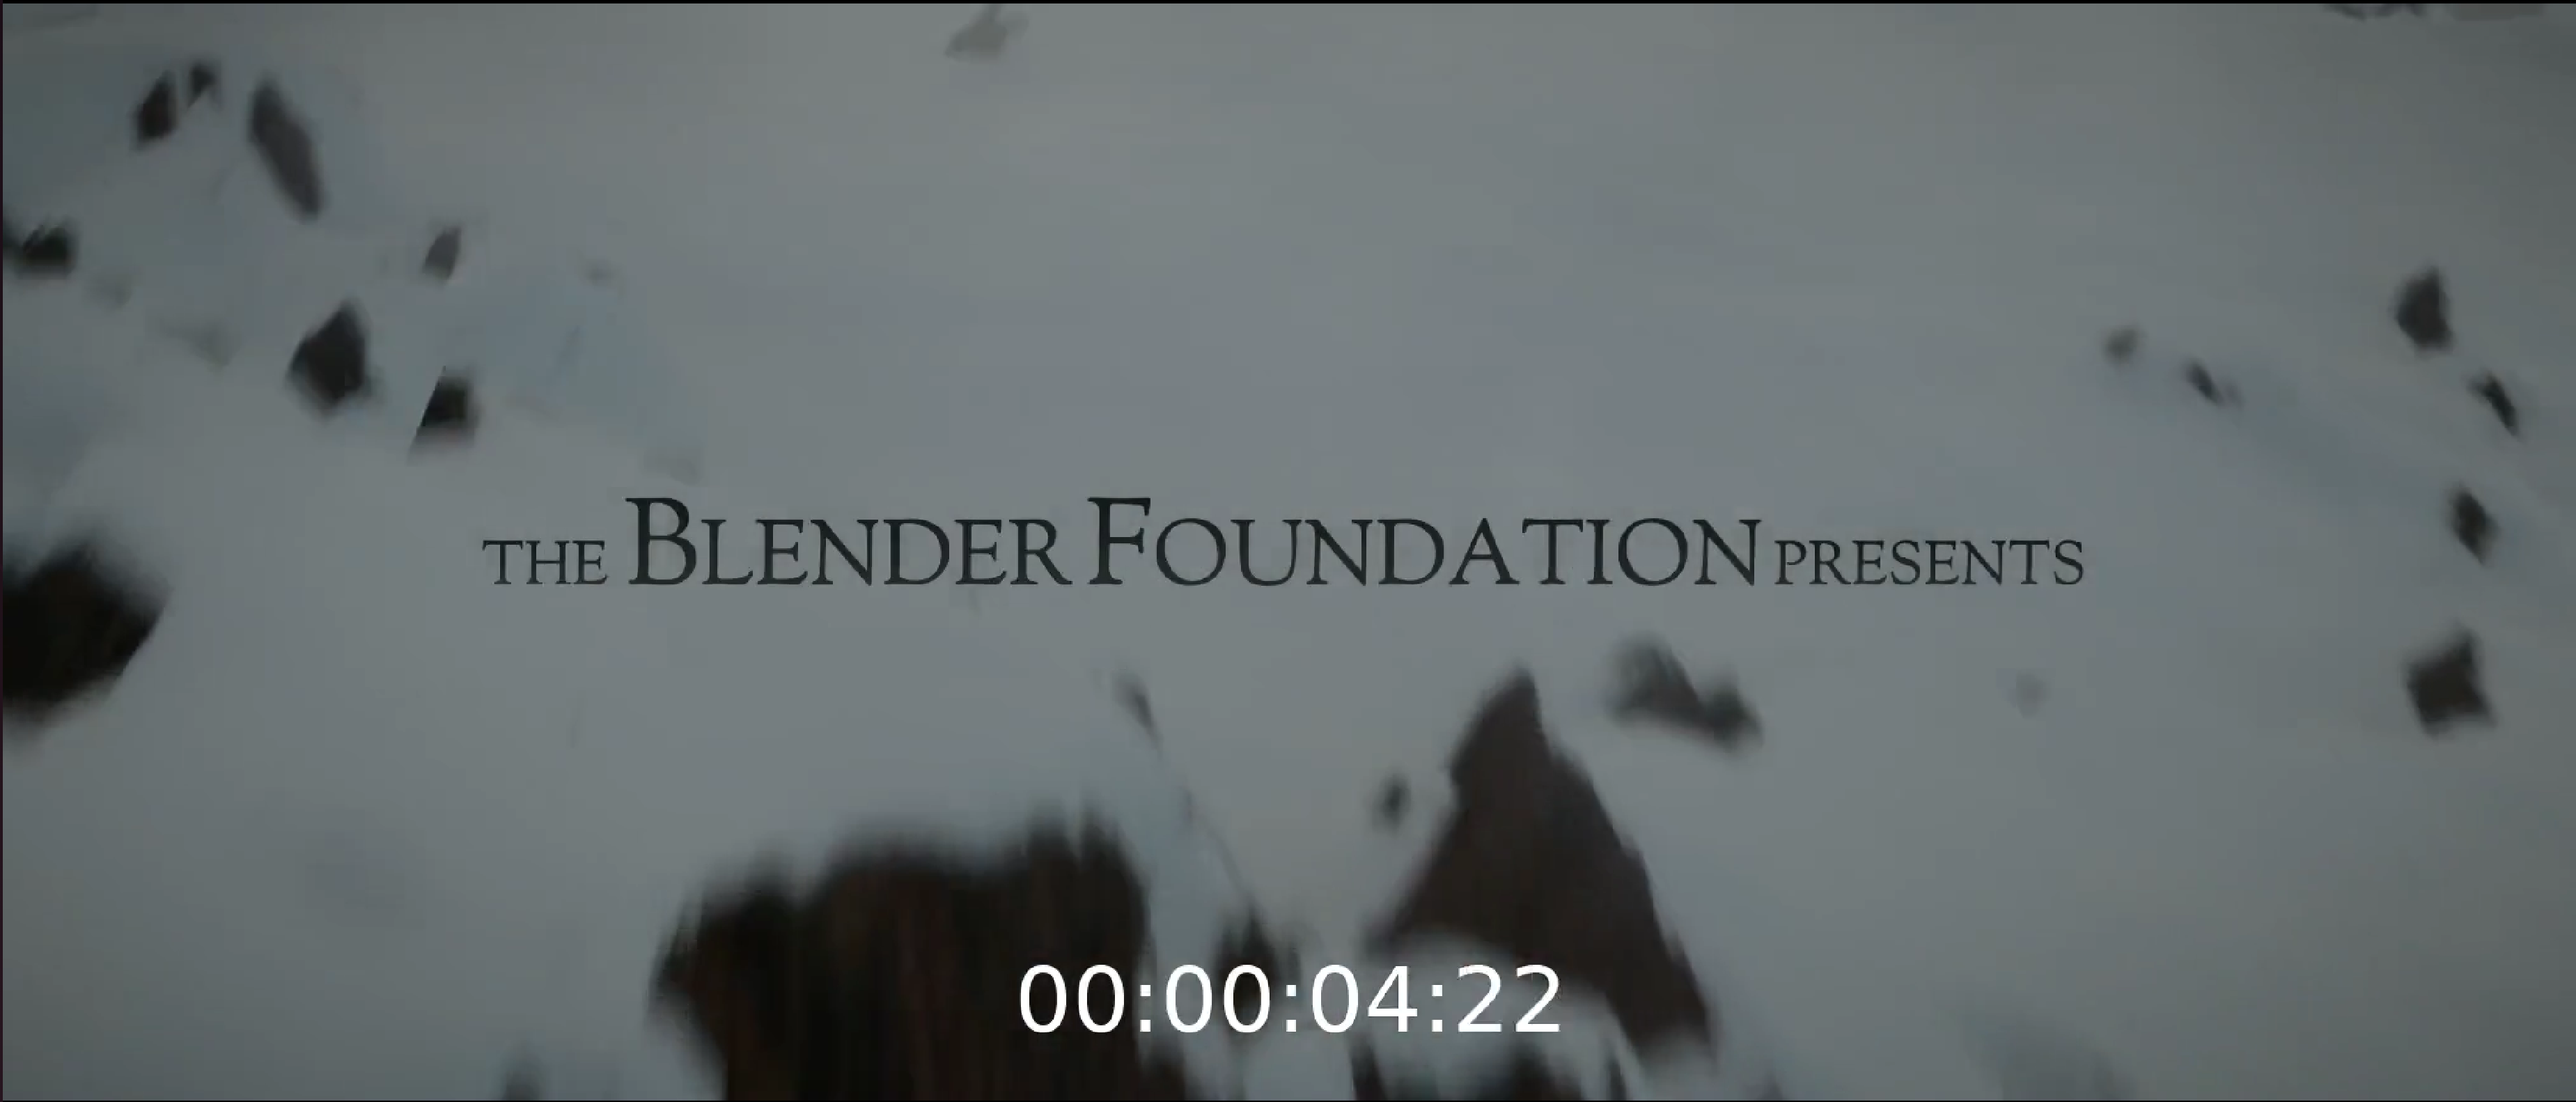
\includegraphics[width=0.9\textwidth]{colourdefault.png}
			Original colours
		\end{minipage}\begin{minipage}{0.5\textwidth}
			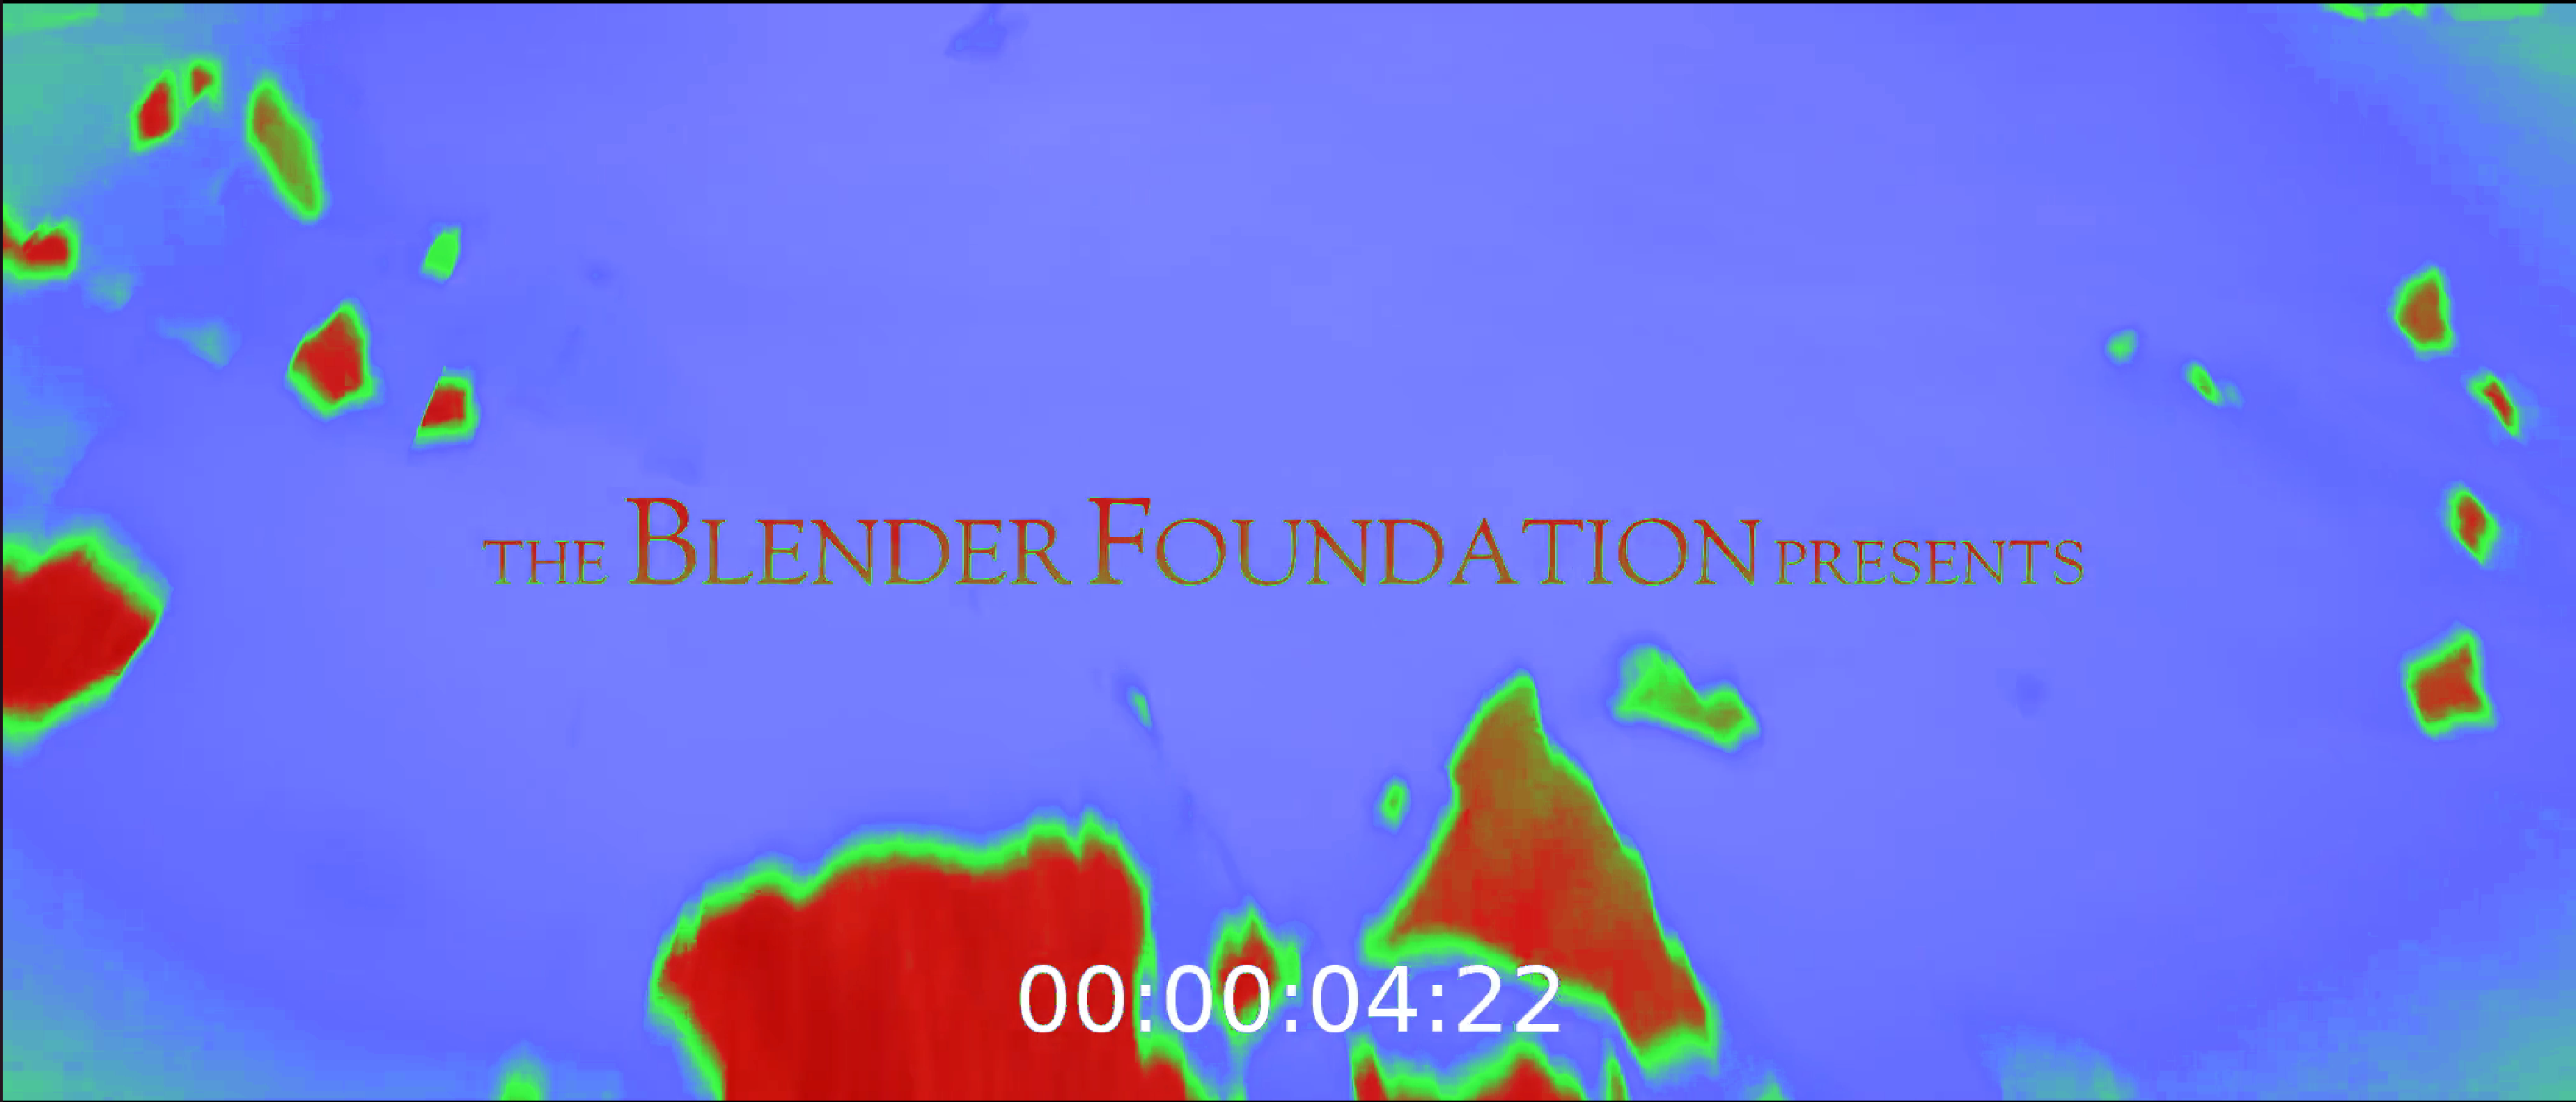
\includegraphics[width=0.9\textwidth]{colourhigh.png}
			Colours with \texttt{av.rs=1} \texttt{av.gm=1} \texttt{av.bh=1}
		\end{minipage}
		
		Float parameters with komma instead of dot, f.ex. $0,5$
		
		Adding filter to \texttt{local\_melt.py} to execute it in the Accurate Player using JIT:
		
		\begin{center}
			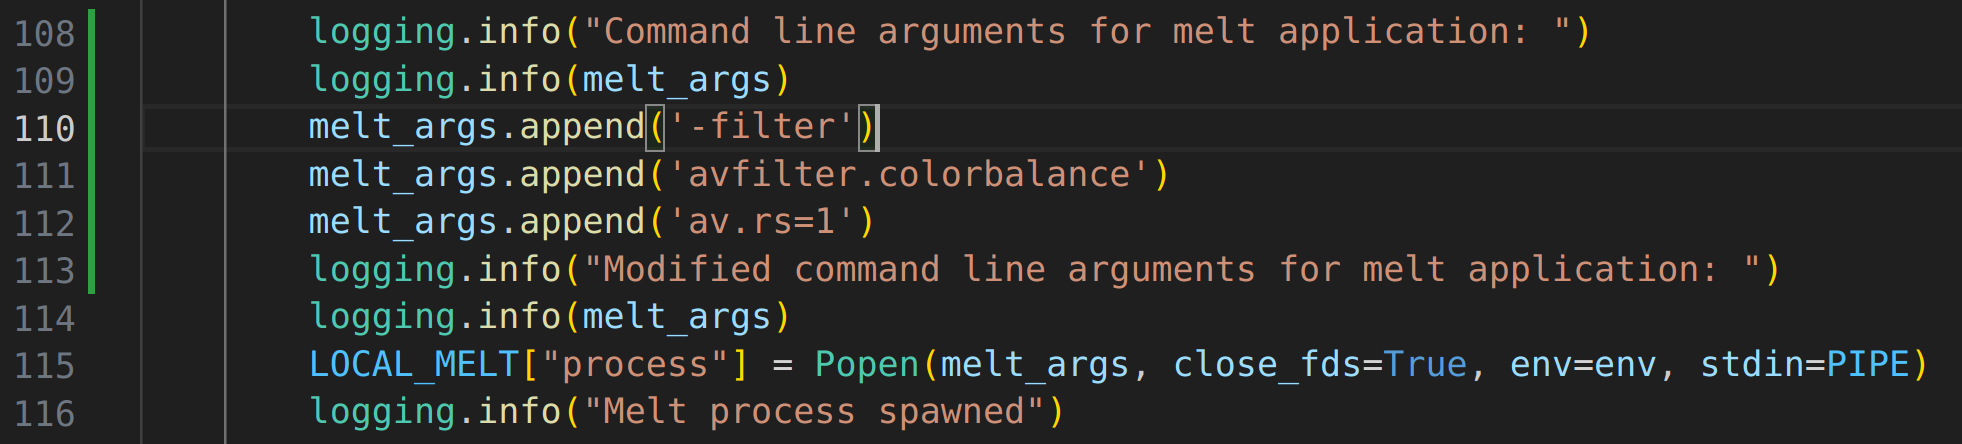
\includegraphics[height=0.13\linewidth]{code.png}
			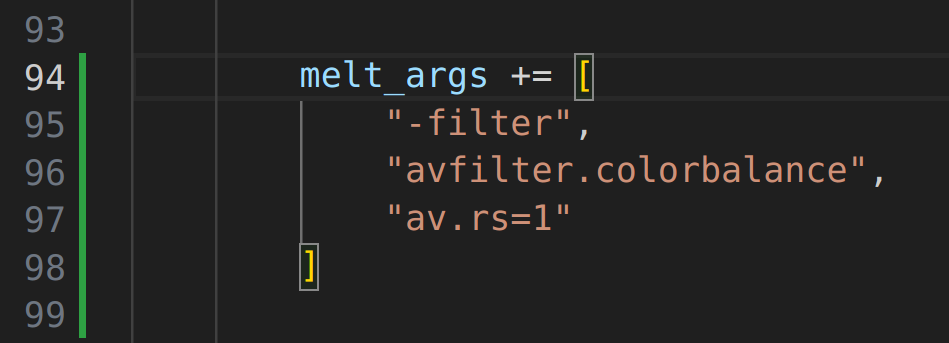
\includegraphics[height=0.13\linewidth]{codecleaner.png}
		\end{center}
		
		\begin{center}
			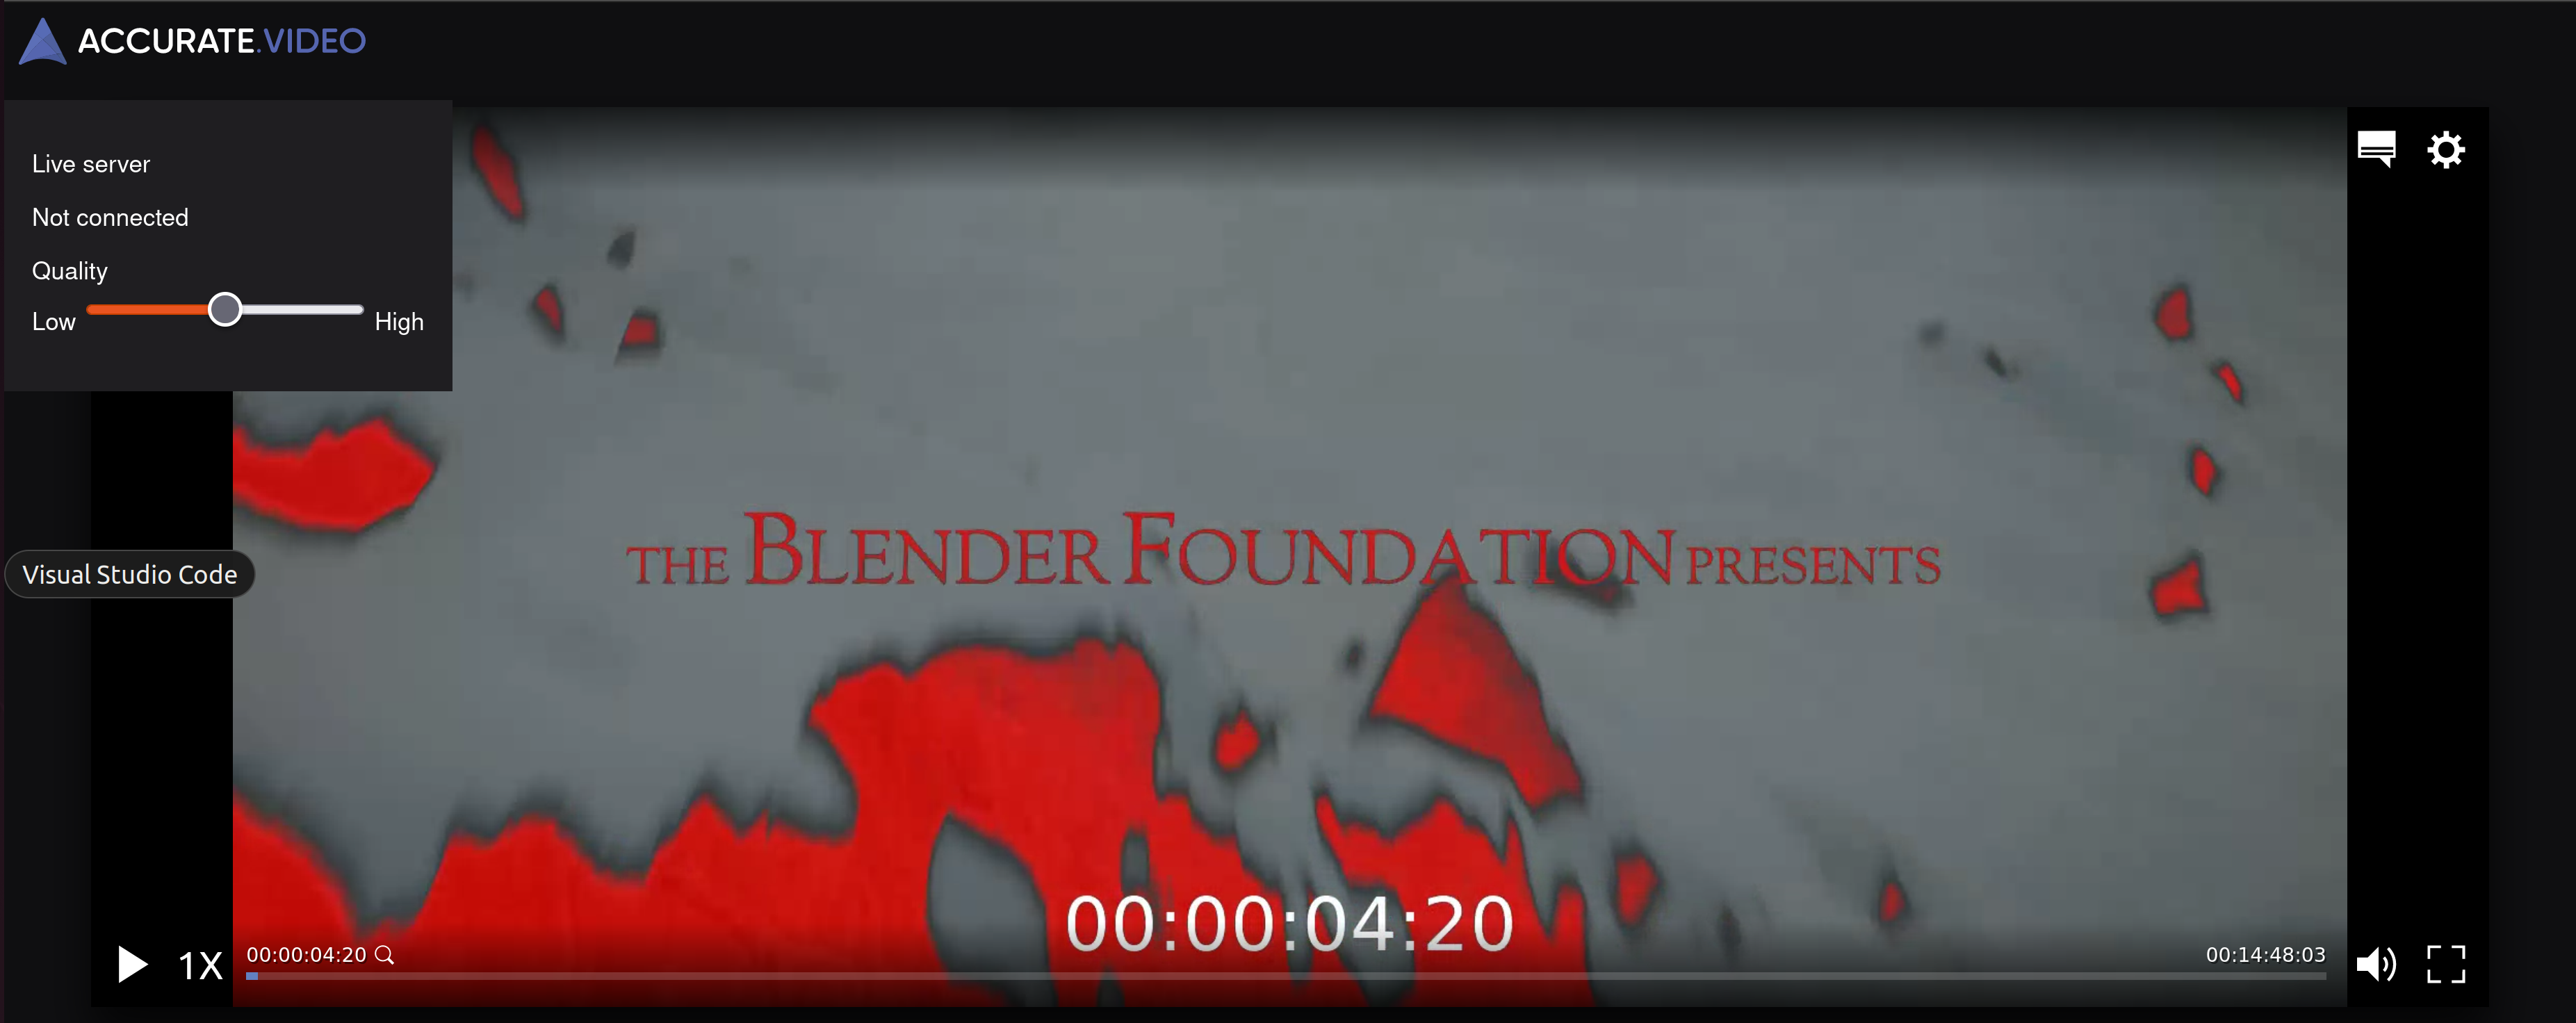
\includegraphics[width=0.8\textwidth]{ap_red.png}
		\end{center}
		

	
		\newpage
		
		\begin{itemize}	
		
		\item \texttt{avfilter.colorchannelmixer}
		
		\url{https://www.mltframework.org/plugins/FilterAvfilter-colorchannelmixer/}
		
		\texttt{title: colorchannelmixer \newline
			media types: Video \newline
			description: Adjust colors by mixing color channels.}
		
		$\rightarrow$ looks promising
		
		
		

		

		
		\item \texttt{avfilter.colorcontrast}
		
		\url{https://www.mltframework.org/plugins/FilterAvfilter-colorcontrast/}
		
		\texttt{title: colorcontrast \newline
			media types: Video \newline
			description: Adjust color contrast between RGB components.}
		
		$\rightarrow$ looks kind of promising
		
		
		%\item avfilter.colorcorrect
		%$\rightarrow$ No -- for black and white balancing
		
		%\item avfilter.colorhold
		%$\rightarrow$ No -- turns a certain color range into gray
		
		%\item avfilter.colorize
		%$\rightarrow$ No -- overlay a solid color on the video stream
		
		%\item avfilter.colorkey
		%$\rightarrow$ No -- turns a certain color into transparency
		
		\item \texttt{avfilter.colorlevels}
		
		$\rightarrow$ Maybe -- Adjust the color levels with black point and white point.
		(The Black point is the Darkest set of pixels in an image, while the White point is the Brightest.)
		
		
		%\item avfilter.colormatrix
		%$\rightarrow$ No
		
		%\item avfilter.colorspace
		%$\rightarrow$ No	
		
		\item \texttt{avfilter.colortemperature}
		$\rightarrow$ Maybe -- adjust color temperature of video.
		
		
		%\item avfilter.pseudocolor
		%\item avfilter.selectivecolor
		%\item[]
		\item \texttt{frei0r.coloradj\_RGB}
		
		\url{https://www.mltframework.org/plugins/FilterFrei0r-coloradj_rgb/}
		
		\texttt{title: coloradj\_RGB \newline
			media types: Video \newline
			description: Simple color adjustment}
		
		$\rightarrow$ looks promising
		
		
		% \item frei0r.colordistance
		% \item frei0r.colorhalftone
		\item \texttt{frei0r.colorize}
		
		\url{https://www.mltframework.org/plugins/FilterFrei0r-colorize/}
		
		\texttt{title: colorize \newline
			media types: Video \newline
			description: Colorizes image to selected hue, saturation and lightness}
		
		$\rightarrow$ looks promising
		
		
		% \item frei0r.colortap
		% \item frei0r.contrast0r
		% \item frei0r.three\_point\_balance
		%\item[]
		%\item tcolor
	\end{itemize}


	% \item[]
	%\item Good to know: \url{https://www.mltframework.org/doxygen/annotated.html}
\end{itemize}



\newpage

\begin{spacing}{1}
	\printbibliography
\end{spacing}
	
	
	
\end{document}